% Charlotte Geiger - Manuel Lippert - Leonard Schatt
% Physikalisches Praktikum

% 3.Kapitel  Protokoll

% Variables
\def\skalierung{0.65}

\chapter{Messprotokoll}
\label{chap:protokoll}

Das Messprotokoll wurde am Versuchstag handschriftlich erstellt und hier als
PDF-Datei eingefügt. Dabei wurden Durchführung und Aufbau schon vorher in dieses
Dokument beschrieben, je nachdem.

% Einbindung des Protokolls als pdf (mit Seitenzahl etc.)
% Erste Seite mit Überschrift
%\includepdf[pages = 1, landscape = false, nup = 1x1, scale = \skalierung , pagecommand={\thispagestyle{empty}\chapter{Protokoll}}]
%            {03 Protokoll/Protokoll.pdf}
% Restliche Seiten richtig skaliert
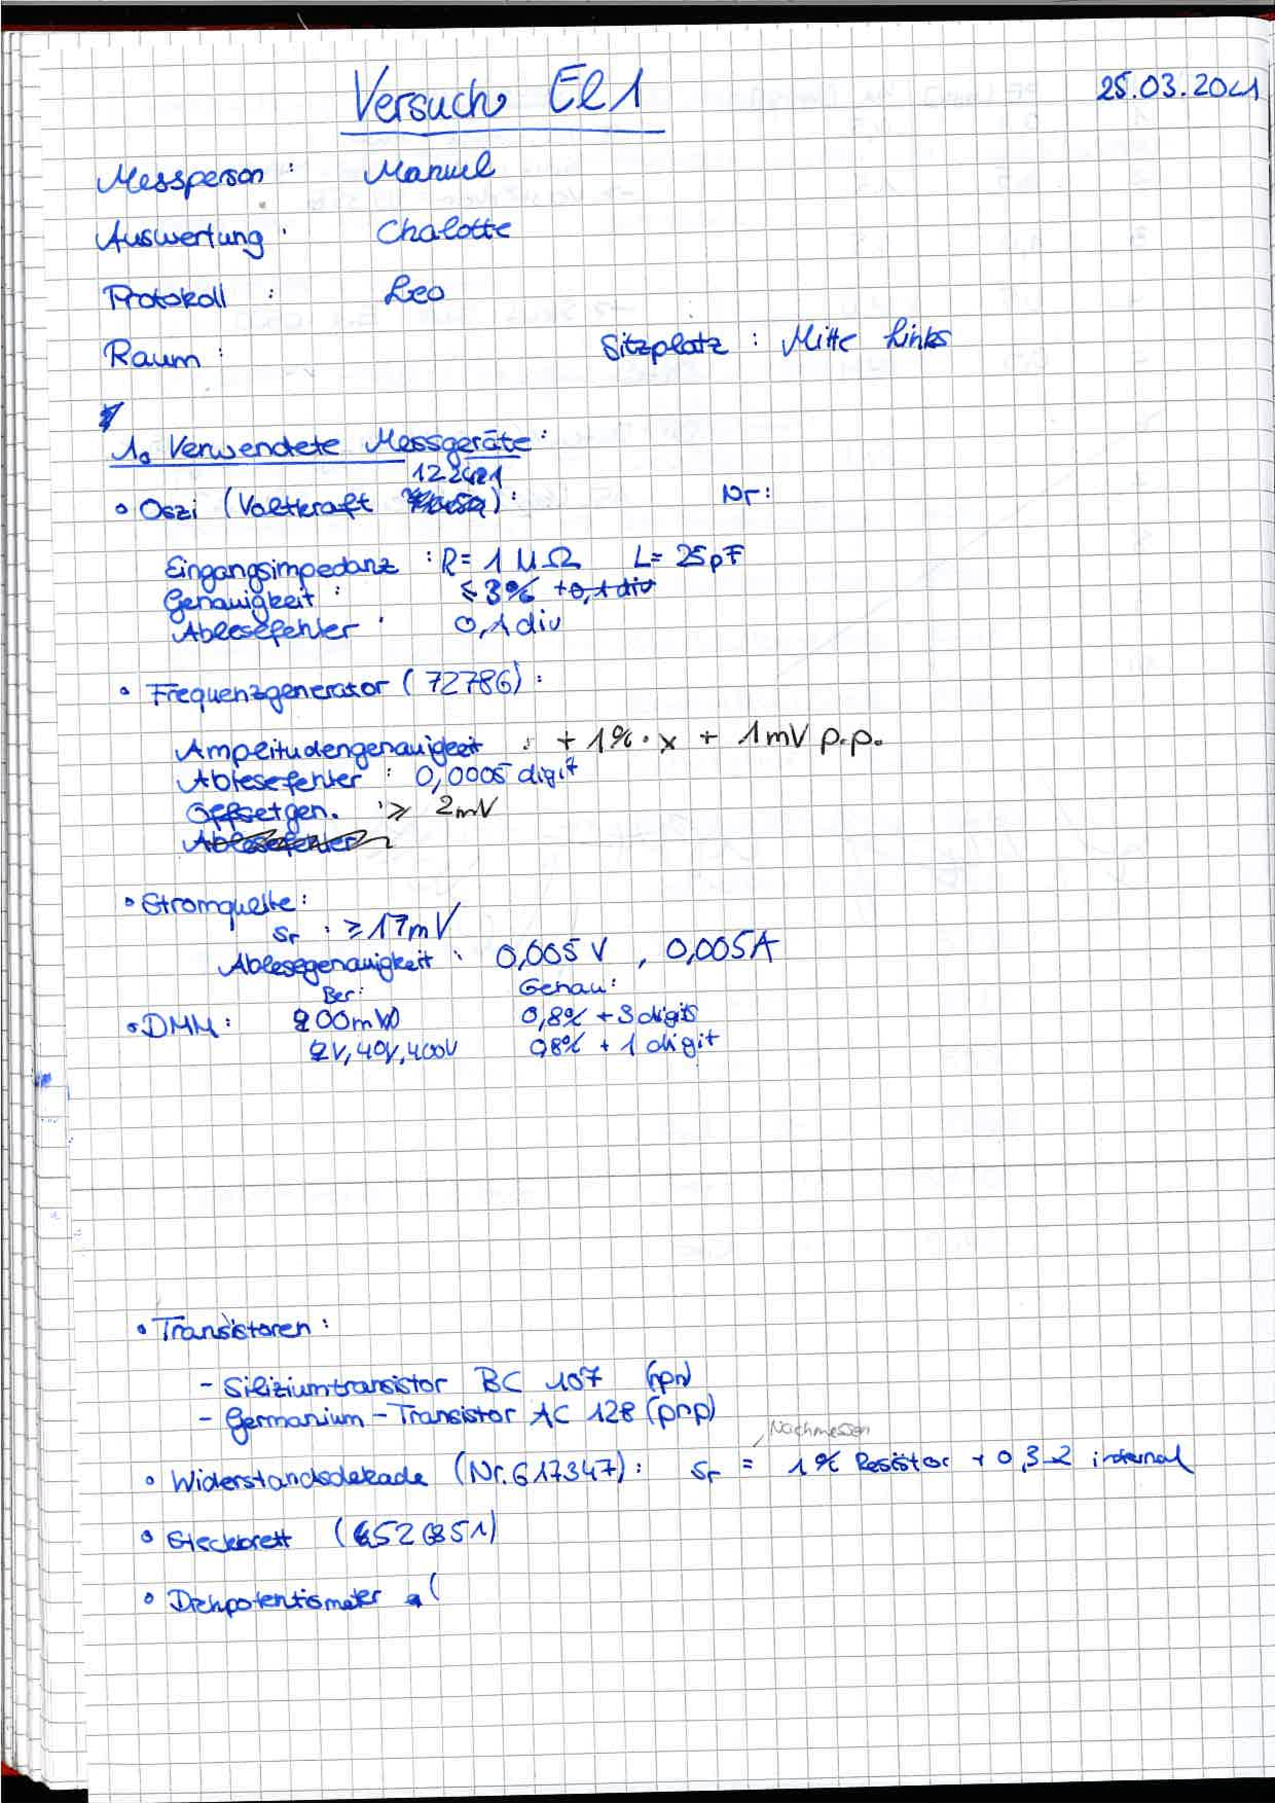
\includepdf[pages = -, landscape = false, nup = 1x1, scale = \skalierung , pagecommand={}]
            {03-Protokoll/Protokoll_EL1.pdf}

%TODO #7 @ManeLippert 
%TODO #10 @ManeLippert